\section*{Introduction}
Stochastic algorithms for the  generation of fractal terrains has a considerable interest in computer graphics, because of their ability to mimic the behaviour of natural terrain.
The applications of fractal terrains is not limited to the generation of  terrain, but includes the generation of clouds, textures, noise and image filters.
In this project we provide and compare three different algorithms that generates fractal landscapes on distributed-memory parallel environments using MPI.

The first, {\em Diamond-Square}, is a simple and widely used recursive algorithm designed to compute high resolution height maps given a low resolution one.
Then we introduce a little-known algorithm that we call {\em Linear Displacement}, that is an attempt to avoid the recursiveness of Diamond-Square.
Finally we discuss an algorithm that uses the {\em Fast Fourier Transform} to do the transform of pink noise, that has an amplitude of $1/f^\alpha$.

\section{Diamond-Square}
\subsection{Sequential algorithm}
Fractal terrain generation can be achieved using the Diamond-Square algorithm introduced by Fournier, Fussel, Carpenter\cite{fournier1982computer} and Miller\cite{miller1986definition}. This algorithm computes a high resolution terrain through multiple iterations, each containing a \textit{square} and \textit{diamond} pass.

The final resolution is as follows:

\begin{equation}
(width_K, height_K) = 2^{K} ((width_0, height_0) - 1) + 1
\end{equation}

With \textit{L} the terrain width or height and \textit{K} the number of iterations. Therefore, each iteration increases the resolution according to $L_{k+1} = 2 L_k - 1$.

Note that if we don't use an initial terrain, $2^K = L$.

\begin{figure}[!htb]
\minipage{0.5\textwidth}
    \centering
    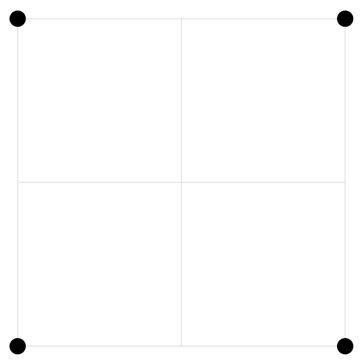
\includegraphics{img/ds_init.jpg}
    \caption{Initial matrix}
\endminipage\hfill
\minipage{0.5\textwidth}
    \centering
    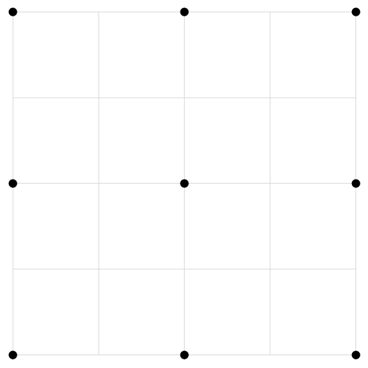
\includegraphics{img/ds_final.jpg}
    \caption{Matrix after the first iteration}
\endminipage\hfill
\end{figure}

To reduce the computation time, we have optimized the memory management by removing the memory allocation and release required by the change of matrix dimensions. Hence, we use a single matrix which has the final terrain dimension. This matrix is actually a simple height map. However, to simplify the algorithm, each iteration only consider a \textit{virtual} matrix which is a part of the final matrix. This matrix has the size expected at the end of the iteration, and we use the following formula to switch from virtual to real matrix coordinates:

\begin{equation}
(i_K, j_K) = 2^{K - k} (i_k, j_k)
\end{equation}

\subsubsection{Randomness}
In order to make our terrain less smooth and thereforemore more realistic, we add a random factor when computing the new points of our terrain.

The random factor \textit{r} is generated according to $0 \leq r \leq scale_k$, with $scale_{k+1} = \frac{scale_k}{2}$.


\subsubsection{Square pass}
The square pass aims at computing the value located at the center of a \textit{square}. This value is the average of those four points.

\begin{equation}
m(i, j) = \frac{m(i-1, j-1) + m(i-1, j+1) + m(i+1, j-1) + m(i+1, j+1) + r)}{4}
\end{equation}

\begin{figure}[H]
\centering
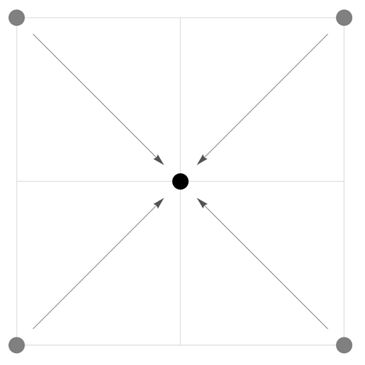
\includegraphics[width=0.3\textwidth]{img/ds_square.jpg}
\caption{Square pass}
\end{figure}

\subsubsection{Diamond pass}
In a similar way, the diamond pass computes the average of four other points as described in figure \ref{fig:ds_diamond}.

\begin{equation}
m(i, j) = \frac{m(i-1, j) + m(i+1, j) + m(i, j-1) + m(i, j+1) + r)}{4}
\end{equation}

\begin{figure}[H]
\centering
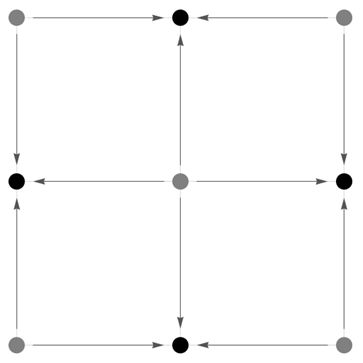
\includegraphics[width=0.3\textwidth]{img/ds_diamond.jpg}
\caption{Diamond pass}
\label{fig:ds_diamond}
\end{figure}


\subsubsection{Water level}
Optionally, every value in the height map below a certain thresold can be set to this threshold after the \textit{K} iterations. This operation can be considered as pouring water on the terrain to give a more realistic rendering.


\subsection{Parallelization}
\subsubsection{Processes topology}
In order to make our program more user friendly, this one takes as input the number of processes \textit{N} and computes the best processes topology $P Q$. This is achieved by computing the two highest factors such that $N = P Q$.

A process coordinates $(p, q)$ in the processes topology is therefore
\begin{equation}
\begin{split}
p = rank \mod P\\
q = \frac{rank}{P}
\end{split}
\end{equation}

While its rank is $rank = q  P + p$

\subsubsection{Scatter and gather data}
Since $P_0$ is the only process importing and exporting the terrain, this algorithm obviously contain a \textit{scatter} (one-to-all) and \textit{gather} (all-to-one) phase, while data is exchanged between $P_0$ and the other processes. To reduce the amount of data exchanged and the memory consumption, each process (except $P_0$) knows only the part of the terrain which has been assigned to it.

The matrix dimensions of a process given its coordinates in the processes grid is given below, with \textit{N} the number of processes ($\sqrt{N}$ is P if we distribute the data width, Q otherwise). This formula guarantees the best linear data distribution on each axis. For simplification, we use $L = length = width = height$

\begin{equation}
\label{eq:ds_data_complexity}
L = \frac{L + \sqrt{N} - 1}{\sqrt{N}} + 
\mathbbm{1}_{rank < (L + \sqrt{N} - 1) \mod \sqrt{N}}
\end{equation}

\subsubsection{Parallel Diamond-Square}
The Diamond-Square algorithm computed by each process is almost the same as previously described. However, we can observe that the diamond pass requires data from other processes. Since each point located at the border of the matrix must be computed based on the values computed by the square pass of two different processes, those \textit{ghost cells} must be exchanged at the end of each iteration using a two-dimensions red-black communication.

The data exchanged only contain $\frac{L_k - 1}{2}$ data points, i.e. the output of the previous square pass for the corresponding terrain side.

\begin{figure}[H]
\centering
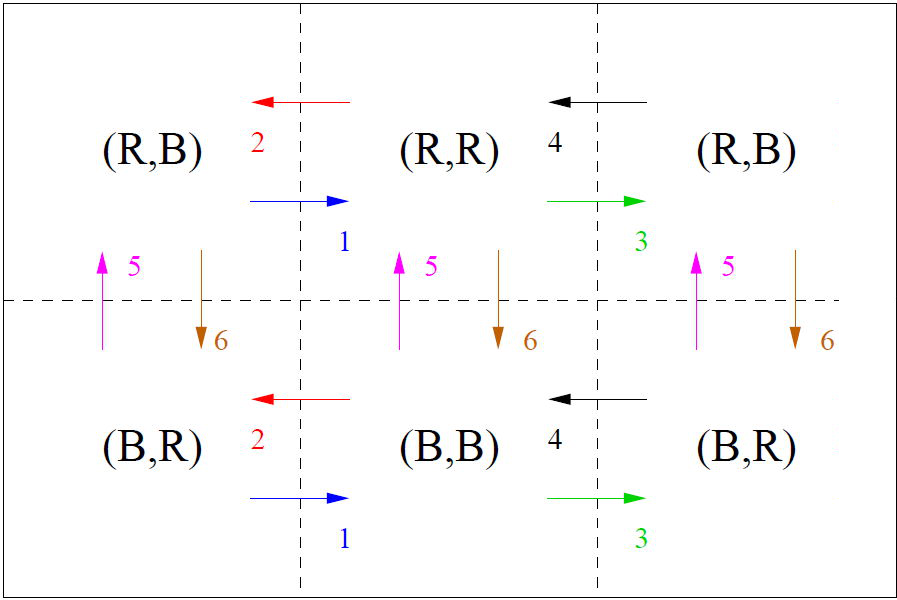
\includegraphics[width=0.6\textwidth]{img/ds_red_black.png}
\caption{Red-Black communication algorithm}
\end{figure}

Since the diamond pass computation also includes a random factor, this one is added to the ghost cells sent by a left-rigth or up-down communication so that each process work with the same data.

After this communication step, the diamond pass is finalized by computing the data points on the four sides of the height map.


\subsubsection{Parallel algorithm}
The parallelized algorithm is eventualy
\begin{lstlisting}
initMPI(argc, argv, &N, &rank);

// Computes the process topology and return the process coordinates
getProcessTopology(N, &P, &Q, &p, &q); 

// Read the initial matrix from an input file then send to each process the part it has to compute
data = importAndScatterData(rank, inputFile, &height, &width, &initWidth, &initHeight, iterations, P, Q);

// Diamond-Square algorithm, including data exchange
diamondSquare(data, initWidth, initHeight, iterations, p, q, P, Q);

// Pour water on the terrain so that every point below the water level is raised to this level
pourWater(data, height, width);

// Gather final data from every process then complete the data matrix for final result
gatherData(data, height, width, rank, P, Q, iterations);

if(rank == 0) {
    // Export the final terrain in the output file
    exportData(data, FINAL_TERRAIN_HEIGHT, FINAL_TERRAIN_WIDTH, outputFile);
}

// Release memory and finalizes MPI
clear(data, height);
\end{lstlisting}

\begin{figure}[!htb]
\minipage{0.5\textwidth}
    \centering
    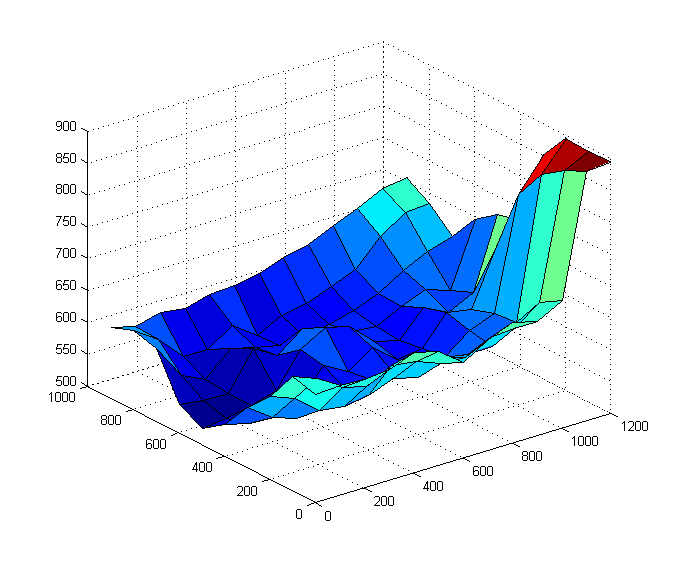
\includegraphics[width=\linewidth]{img/init.png}
    \caption{Initial terrain (13x10)}
\endminipage\hfill
\minipage{0.5\textwidth}
    \centering
    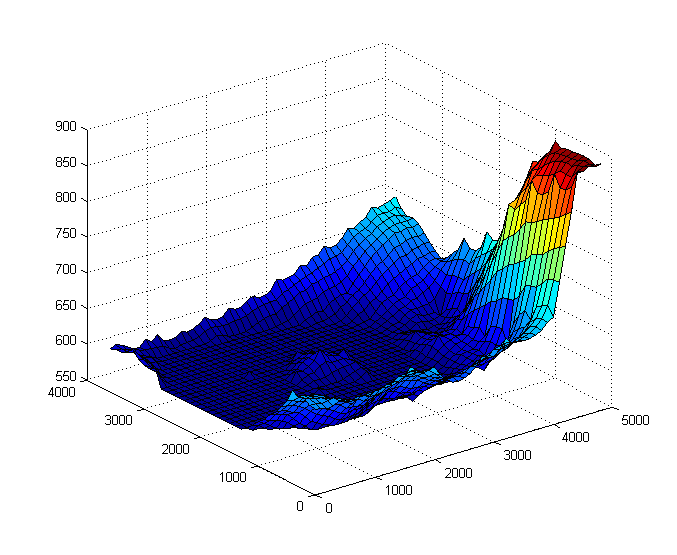
\includegraphics[width=\linewidth]{img/final.png}
    \caption{Final terrain - 2 iterations (49x37)}
\endminipage\hfill
\end{figure}

\subsection{Parallel efficiency}
\subsubsection{Complexity}
The complexity of the Diamond-Square algorithm is obtained as follows, assuming a perfectly load balanced linear data distribution, $\sqrt{N} = P = Q$
Seeing that  for the {\em Diamond-Square} step we have a complexity of

\begin{multline}
\underbrace{\order\left((N-1) \left(\frac{L_0 + N - 1}{\sqrt{N}}\right)^2\right)}_{\text{scatter data}} + \order\left(\sum\limits_{k = 1}^{K} \text{square} + \text{diamond} + \text{exchange} + \text{update diamonds}\right) +\\+ \underbrace{\order\left((N-1) \left(\frac{L_K}{\sqrt{N}}\right)^2\right)}_{\text{gather data}}
\end{multline}

$L_k$ is the data width or height at iteration k. Hence, $L_K^2$ is the final terrain dimension, with K the total number of iterations. The complexity for an iteration is

\be
\underbrace{
    \underbrace{\order\left(\left(\frac{L_k}{2\sqrt{N}}\right)^2 \right)}_{\text{square}} +
    \underbrace{\order\left(\frac{(L_k/\sqrt{N})^2}{2} \right)}_{\text{diamond}} + 
    \underbrace{\order\left(\frac{4 L_k}{2\sqrt{N}}\right)}_{\text{exchange}} + 
    \underbrace{\order\left(\frac{4 L_k}{2\sqrt{N}}\right)}_{\text{update diamonds}}
 }_{\text{Diamond-Square}}
\ee

We eventually get the total complexity
\begin{equation}
\begin{split}
\order\left(L_0^2 + \sum\limits_{k = 1}^{K} \left(\left(\frac{L_k}{\sqrt{N}}\right)^2 \, + \left(\frac{L_k}{\sqrt{N}}\right)^2 \, + \frac{L_k}{\sqrt{N}}\, + \frac{L_k}{\sqrt{N}}\right) + L_K^2\right)\\
= \order\left(L_0^2 + \sum\limits_{k = 1}^{K} \frac{L_k^2}{N}\right)\\
= \order\left(\frac{L^2}{N}\right)
\end{split}
\end{equation}

This last step is obtained by solving the geometric series for $L_K \approx 2^K$ when starting with an empty terrain.

Eq.~\ref{eq:ds_data_complexity} gives us the data distribution. Based on this equation, the distribution is almost optimal:
\be
\frac{L + \sqrt{N} - 1}{\sqrt{N}} + \mathbbm{1}_{rank < (L + \sqrt{N} - 1) \mod \sqrt{N}} \underset{L\to +\infty}{\longrightarrow} \frac{L}{\sqrt{N}}
\nonumber
\ee

\subsubsection{Benchmarks and speedup}
According to fig.~\ref{fig:benchmarks_ds}, we can observe that our algorithm scales quite poorly. If the computation of the terrain scales quite efficiently, the loss of performances is mostly caused by the important communication cost when gathering data. Indeed, fig.~ \ref{fig:benchmarks2_ds} shows a much more interesting speedup without data gathering.

\begin{figure}[!htb]
\minipage{0.5\textwidth}
    \centering
    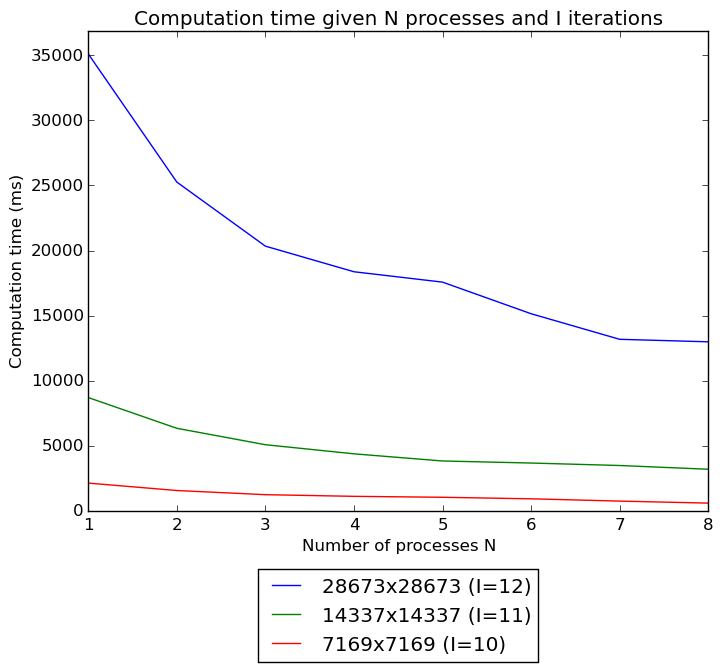
\includegraphics[width=\linewidth]{img/ds_benchmarks1.png}
    \caption{Benchmarks}
    \label{fig:benchmarks_ds}
\endminipage\hfill
\minipage{0.5\textwidth}
    \centering
    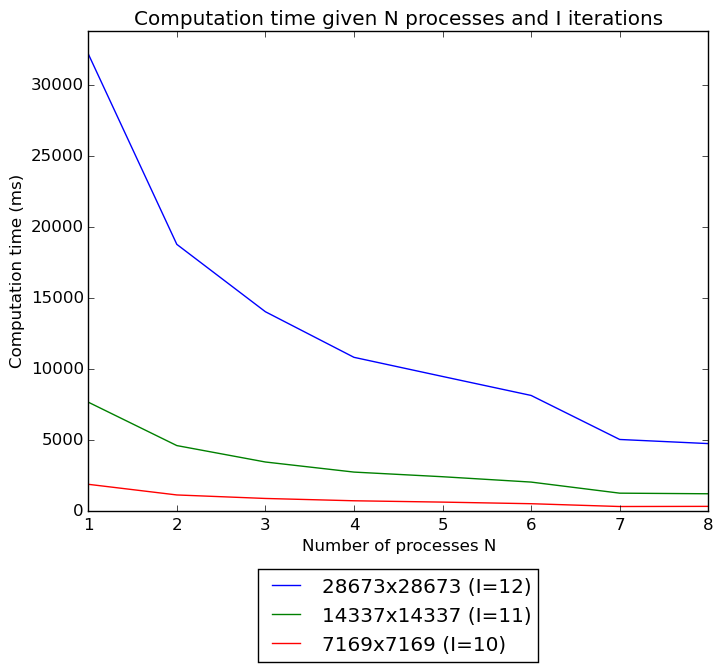
\includegraphics[width=\linewidth]{img/ds_benchmarks2.png}
    \caption{Benchmarks - No data gathering}
    \label{fig:benchmarks2_ds}
\endminipage\hfill
\end{figure}

\pagebreak

Because of the amound of data exchanged at the end of the algorithm, we obtain the speedups for an output resolution of 28673x28673 visible in table~\ref{table:speedup}. We assume $T^{\*}_s \approx T_1$ since our algorithm do not contain any communication or additional computation when $N = 1$.

\begin{table}[H]
\begin{center}
\begin{tabular}{c|c|c|c|c|}
 & \multicolumn{2}{c|}{Gathering} & \multicolumn{2}{c|}{Without Gathering} \\
\hline
Processes & $T_p$ [s] & $S_p$ & $T_p$ [s] & $S_p$ \\

\hline
$2$ & 25.256 & 1.39 & 18.773 & 1.71 \\
$4$ & 18.370 & 1.91 & 10.820 & 2.97\\
$8$ & 12.990 & 2.70 & 4.746 & 6.78\\
\hline
\end{tabular}
\caption{\label{table:speedup} Running time $T_p$ and speedup $S_p$ for different amount of processes. The running time for a single process is $T^{\*}_s = 35.100$~s with gathering and $T^{\*}_s = 32.186$~s without.}
\end{center}
\end{table}




\pagebreak
\FloatBarrier

\section{Linear Displacement}
This algorithm is a simple but non-intuitive method to create fractal terrain. It is used as an example to model realistic planets\cite{paulbourke}, but can be easily be modified to generate rectangular heightmaps.
\subsection{Algorithm}
The approach of our algorithm can be summarized as following:
\bi
    \ib pick a random line going through the heightmap
    \ib  increase or decrease (decide at random) by one the height of each point under the line
    \ib repeat until you are satisfied with the result
\ei
These steps are shown in fig.~\ref{liter}, where we can see the algorithm at an increasing number of iterations.
The algorithm is suprisingly short, yet requires a great deal of iterations to get good results.
In our implementation the line is generated by choosing two random points in the grid and finding the equation of the line that passes through them.
In cartesian coordinates, if $(x_1,y_1)$ and $(x_2,y_2)$ are two independent random points with uniform distribution, then the equation of the line will be
\be
    \frac{y-y_1}{y_2-y_1}=\frac{x-x_1}{x_2-x_1}
\ee
The fact that we lift (or lower) all the points {\em under} this line is irrelevant and does not qualitatively change the terrain.
We could do it for the points {\em over} the line if we wanted to.
The original algorithm\cite{paulbourke}, raises one side and lowers the other, but this requires to access all points in the array at each iteration. 
Our method allows us to access on average only half of the array points, without losing any quality.

Finally a note on the number of iterations: to have a decent quality (no presence of artifacts), we usually need a number of iterations proportional to the number of points
\be\label{Niter}
    N_{iter} = q L_x L_y
\ee
where we define $0<q<1$ as the quality factor. To have acceptable results we empirically take $q\simeq 0.1$.
\subsection{Parallelization}
The parallelisation of this algorithm is quite simple, as the iterations do not depend on each other.
Therefore we split the number of iterations along the processes and, once that is complete, perform a {\tt MPI\_reduce()} to superpose the iterations of the different processes on the root process.

\begin{figure}[h]
\minipage{0.5\textwidth}
    \centering
    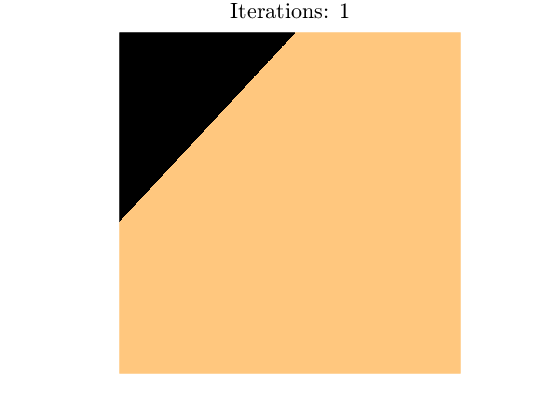
\includegraphics[width=\linewidth]{img/lines1.png}
\endminipage\hfill
\minipage{0.5\textwidth}
    \centering
    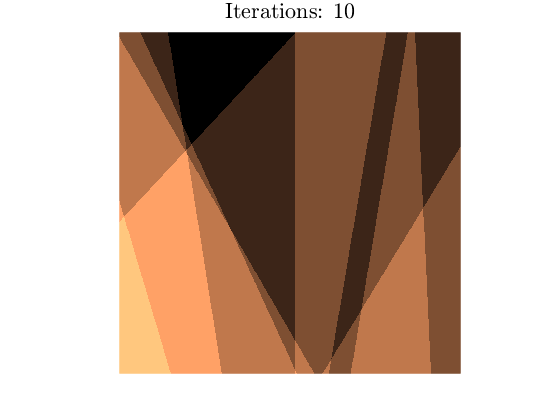
\includegraphics[width=\linewidth]{img/lines1e1.png}
\endminipage\hfill

\minipage{0.5\textwidth}
    \centering
    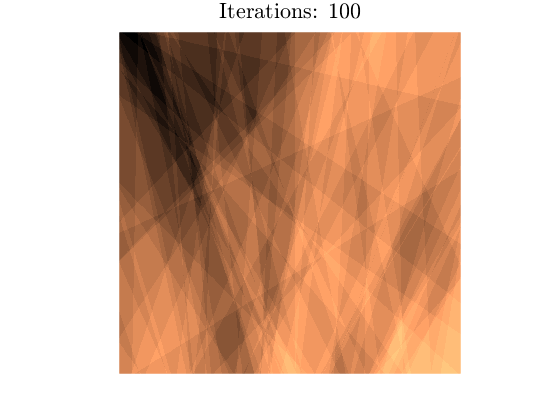
\includegraphics[width=\linewidth]{img/lines1e2.png}
\endminipage\hfill
\minipage{0.5\textwidth}
    \centering
    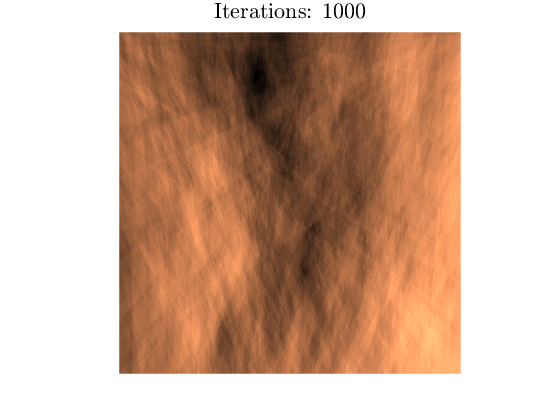
\includegraphics[width=\linewidth]{img/lines1e3.png}
\endminipage\hfill

\minipage{0.5\textwidth}
    \centering
    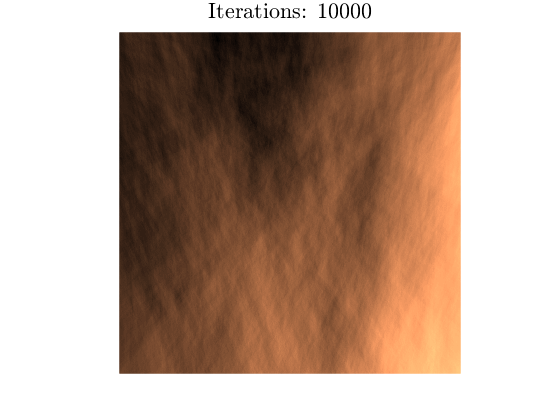
\includegraphics[width=\linewidth]{img/lines1e4.png}
\endminipage\hfill
\minipage{0.5\textwidth}
    \centering
    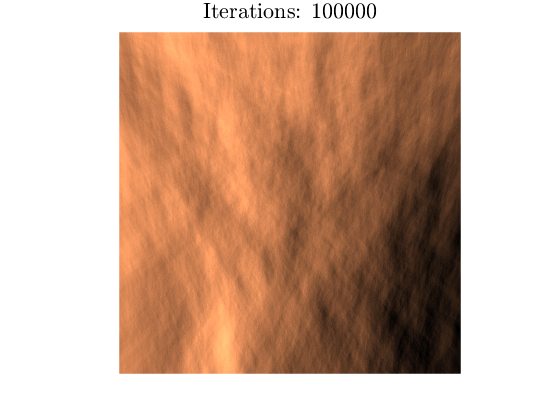
\includegraphics[width=\linewidth]{img/lines1e5.png}
\endminipage\hfill

\caption{\label{liter}Linear displacement algorithm with an increasing number of iterations.}
\end{figure}

\subsection{Performance analysis}
\subsubsection{Complexity}
For simplicity we assume $L = L_x = L_y$.
At each iteration we have to access on average $L^2/2$ points.
But, as discussed before, each process must perform $N_{iter}/N$ iterations.
Thus, by eq~\ref{Niter} we have a complexity of 
\be
    \underbrace{\order(q L^2/N) \order(L^2/2)}_{\text{iterations}} + \underbrace{\order(L^2\log{N})}_{\text{reduce}} = \underbrace{\order(L^4/N)}_{\text{overall}}
\ee
since we can safely assume that $N\ll L^2$. 

We remark that this algorithm is considerably slower as it does not scale as well as the other ones we present. However the constant hidden behind the $\order$ notation is considerably small --- we simply increment the value of a memory location --- making this algorithm  an interesting study case nonetheless.
\begin{figure}[htb]
\centering
    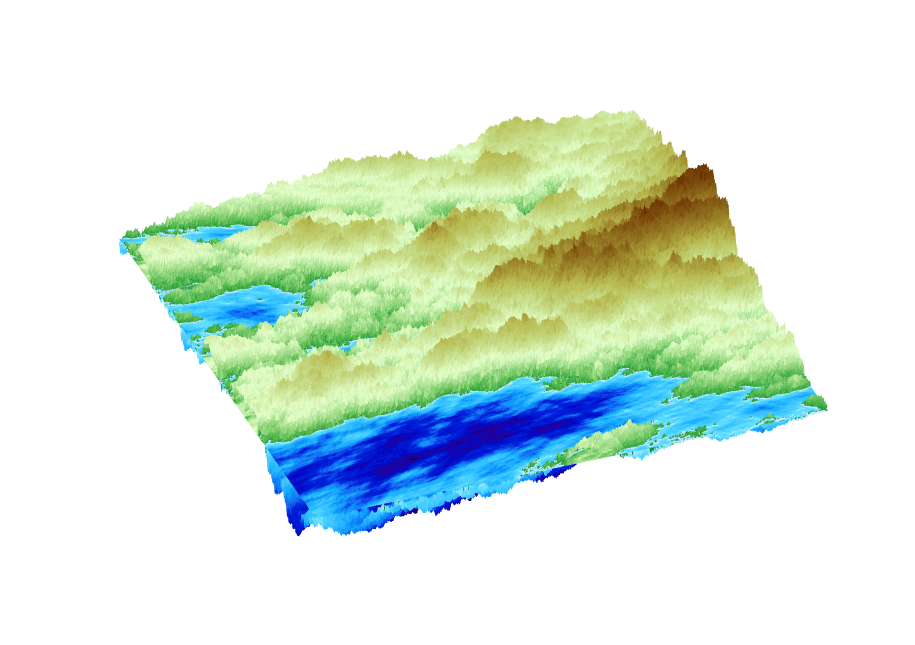
\includegraphics[width=0.8\textwidth]{img/lines3d.png}
    \caption{\label{lines3d}Example of terrain generated with the lines displacement algorithm}
\end{figure}

A tipical result is presented in fig.~\ref{lines3d}. We notice that the peaks are quite jagged. 
One feature of this algorithm is that it does not take any parameter to control the ``smoothness'' of the fractal.

\subsubsection{Experimental results}

Runs on the {\em Ferlin} computer at PDC confirm that this algorithm is significantly slower than the other two presented. For this reason the benchmarking has been done with significantly lower sizes.

\begin{figure}[!htb]
\minipage{0.5\textwidth}
    \centering
    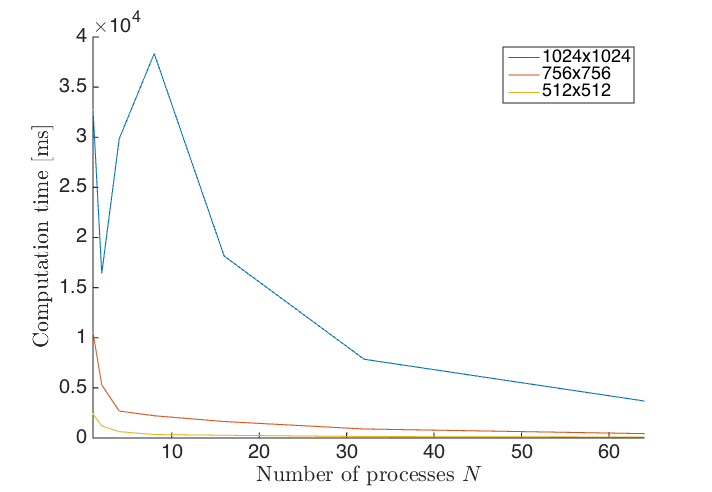
\includegraphics[width=\linewidth]{img/lines_benchmarks1.png}
    \caption{Execution time for the linear displacement algorithm}
    \label{fig:benchmarks_time_ld}
\endminipage\hfill
\minipage{0.5\textwidth}
    \centering
    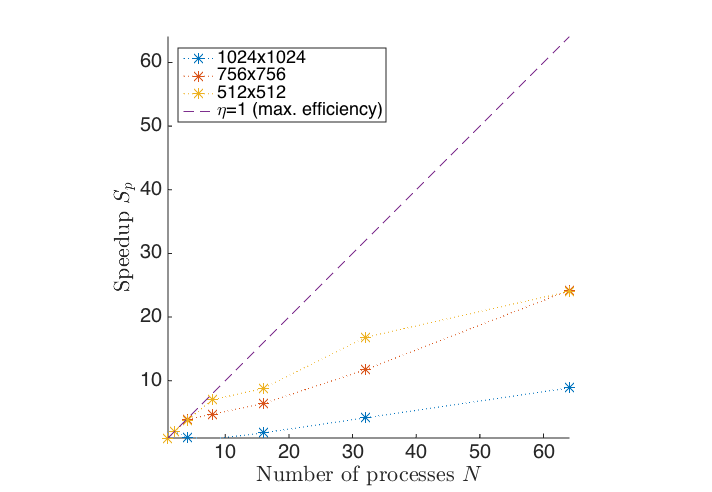
\includegraphics[width=\linewidth]{img/lines_benchmarks2.png}
    \caption{Speedup for the linear displacement algorithm}
    \label{fig:benchmarks_speedup_ld}
\endminipage\hfill
\end{figure}

By inspecting the performance results in fig.~\ref{fig:benchmarks_time_ld} and fig.~\ref{fig:benchmarks_speedup_ld} we see that the performance is very sensitive to the number of processes and the efficiency actually goes down with the size of the height map.
This suggest that the major bottleneck is the communication step, where the processes communicate a very large amount of data.

The data collected is summarized in table~\ref{table:speedup_ld}, along with the average speedup.

\begin{table}[H]
\begin{center}
\begin{tabular}{c|c|c|c|c|}
$L$ =  & 512 & 756 & 1024 &  \\
\hline
Processes & \multicolumn{3}{c|}{$T_p$ [s]} & {$\bar{S_p}$} \\
\hline
$2$ & 1.2160 & 5.2860 & 16.4160 & 1.98\\
$4$ & 0.6330 & 2.6900 & 29.8530 & 2.94\\
$8$ & 0.3430 & 2.2200 & 38.3460 & 4.20\\
$16$ & 0.2730 & 1.6430 & 18.1460 & 5.67\\
$32$ & 0.1430 & 0.9000 & 7.8560 & 10.9\\
$64$ & 0.1000 & 0.4360 & 3.6960 & 19.0\\

\hline
\end{tabular}
\caption{\label{table:speedup_ld} Running time $T_p$ and average speedup $\bar{S_p}$ for different amount of processes and sizes.}
\end{center}
\end{table}




    
\pagebreak
\FloatBarrier

\section{Fast Fourier Transform}
Fractal terrain generation with a Discrete Fourier Transform has been experimented previously\cite{koh1992fast}.
The idea is to do the inverse transform of pink noise to generate a terrain.
This can be done very quickly with a {\em Fast Fourier Transform} (which will be later referred as FFT). In order to do so, in our parallel implementation we use the {\em FFTW}\cite{fftw} library.
\subsection{Algorithm}
In the first step each process initially generates it's share of complex coefficients with a pink noise damping. This means that in frequency space we have
\be
    P(x_i,y_j) = \frac{z}{(x_i^2+y_j^2)^{\alpha}}
\ee
where $0<\alpha<2$ is a parameter that will determine the roughness of the terrain, and $z$ is a random complex number with a normal distribution.
Since C {\tt stdlib.h} library generates uniformly distributed floating point numbers, this is done with a Box-Muller tranform. 
This is done by taking two independent random variables with a uniform distribution in the range $(0,1)$, say $u_1$ and $u_2$. Then we can generate a complex number $z$ with a normal distribution as following
\be
    z = \sqrt{-2 \ln{u_1}} \exp(2\pi i u_2)
\ee
Since the full height map will be a $L_x L_y$ matrix, each process with have a slice of $L_x L_y / N$ points, where $N$ is the total number of processes used. 

The second step of the algorithm is to perform a parallel FFT  of the points we generated in frequency space. 
In theory we should do an inverse fourier transform, but we can do a direct transform, but this does not change the result qualitatively. 
It also saves some computations as it saves us from a rescaling factor.
The transform is handled by the FFTW library, that has an MPI implementation.
The advantage of this configuration is that the matrix is distributed along the processes, so that the algorithm can handle arrays that are too big to fit on a single process.
The disadvantage of performing an FFT on a distributed memory system is that the algorithm requires to do a transpose, which involves a {\em complete exchange}: each process must communicate to all the others.

Finally, each process writes in order their results to {\tt stdout}; in a tipical usage the user will redirect this output to a file or to {\tt /dev/null} for benchmarking.

One property of this algorithm is that, because of the periodicity of the Fourier transform, it can tiled. As can seen in fig.~\ref{fig:fft3d} the algorithm generates more  ``rolling hills'', due to the smoothness and continuity of the $\sin$ or $\cos$ functions.
\begin{figure}[htb]
\centering
    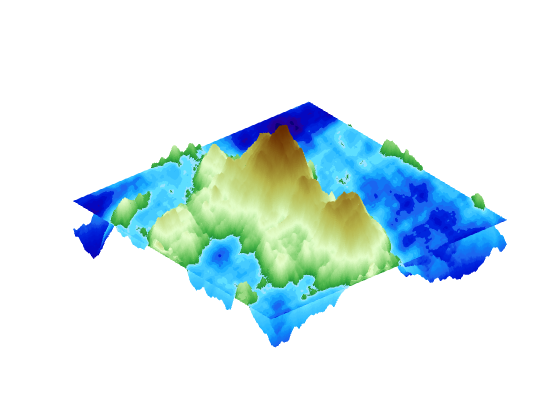
\includegraphics[width=0.8\textwidth]{img/fft3d.png}
    \caption{\label{fig:fft3d}Example of terrain generated with the FFT algorithm ($\alpha=1.1$)}
\end{figure}

\subsection{Performance analysis}
\subsubsection{Complexity}
As before we will estimate the complexity with  a square height map ($L = L_x =  L_y$) with $N$ processes. Since we do not know exactly the complexity of the FFTW routine, but we can estimate that at worst it runs in times comparable to a 2D Cooley-Tuckey algorithm. Therefore, ignoring writing times we have 
\be
    \underbrace{\order(L^2/N)}_{\text{init. of coeffients}} + \underbrace{\order((L \log L)^2/N)}_{FFT} = \underbrace{\order(L^2 \log^2 L/N)}_{\text{overall}}
\ee
\subsubsection{Experimental results}
The benchmarking from parallel runs on the {\em Ferlin} machine using a  number of processes that are powers of 2, for which the FFT is most performant. 
The results are presented in fig.~\ref{fig:benchmarks_time_fft}  and fig.~\ref{fig:benchmarks_speedup_fft}, where we can observe the execution times and the speedup for different height map size and different number of processes. 
We remark that the execution times are quite slower compared to the Diamond-Square algorithm, but this algorithm performs impressively well when the scale becomes larger, since the efficiency $\eta$ is close to 1 (see fig.~\ref{fig:benchmarks_speedup_fft}). The data is presented in table~\ref{table:speedup_fft}.


\begin{table}[H]
\begin{center}
\begin{tabular}{c|c|c|c|c|}
$L$ =  & 3584 & 7168 & 14336 &  \\
\hline
Processes & \multicolumn{3}{c|}{$T_p$ [s]} & {$\bar{S_p}$} \\
\hline
$2$ & 2.266 & 14.683 & 62.276 & 1.80\\
$4$ & 1.190 & 7.700  & 32.173 & 3.44\\
$8$ & 0.676 & 4.250  & 17.863 & 6.17\\
$16$ & 0.406 & 1.973 & 9.206 & 11.9\\
$32$ & 0.236 & 0.843 & 5.060 & 23.7\\
$64$ & 0.116 & 0.436 & 2.180 & 49.3\\

\hline
\end{tabular}
\caption{\label{table:speedup_fft} Running time $T_p$ and average speedup $\bar{S_p}$ for different amount of processes and sizes.}
\end{center}
\end{table}

\begin{figure}[!htb]
\minipage{0.5\textwidth}
    \centering
    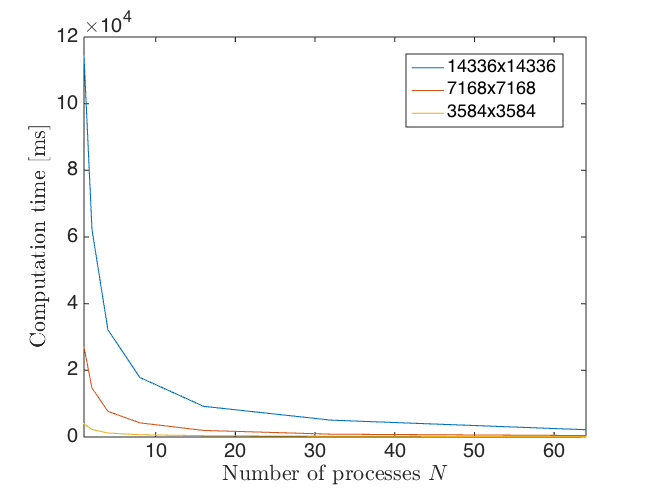
\includegraphics[width=\linewidth]{img/fft_benchmarks1.png}
    \caption{Execution time for the FFT algorithm}
    \label{fig:benchmarks_time_fft}
\endminipage\hfill
\minipage{0.5\textwidth}
    \centering
    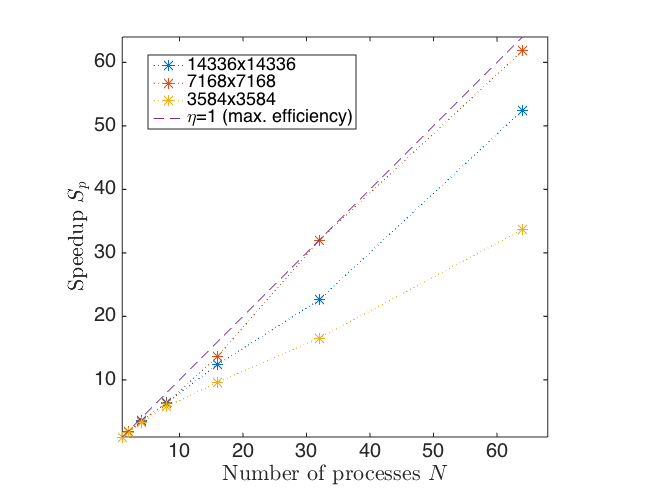
\includegraphics[width=\linewidth]{img/fft_benchmarks2.png}
    \caption{Speedup for the FFT algorithm}
    \label{fig:benchmarks_speedup_fft}
\endminipage\hfill
\end{figure}




\section{Conclusion}
In this work we provided the implementation and discussed three different stochastic algorithms for the generation of fractal landscapes in parallel environments.

The classic Diamond-Square algorithm has the lowest complexity and performed the fastest, although does not scale as nicely in distributed-memory parallel environments due to the fact that there is an increasing amount of communication required between processes. 
The somewhat unusual Linear Displacement algorithm was presented for academic interest, but performs quite poorly both at large scales and in large parallel systems.
Finally, using the Fast Fourier Transform of pink noise we provided an algorithm that is slower than Diamond-Square but behaves more efficiently in large-scale environments, where the data has to be distributed along different memory locations and the number of processes is considerable.

More advanced terrain generations take in account that the fractal properties are not uniform everywhere. A more advanced technique uses {\em multifractal systems} where we combines different fractal algorithms. As a simple experiment we combined the results from the  algorithms we implemented, as can be seen in fig.~\ref{fig:full} \begin{figure}[htb].
\centering
    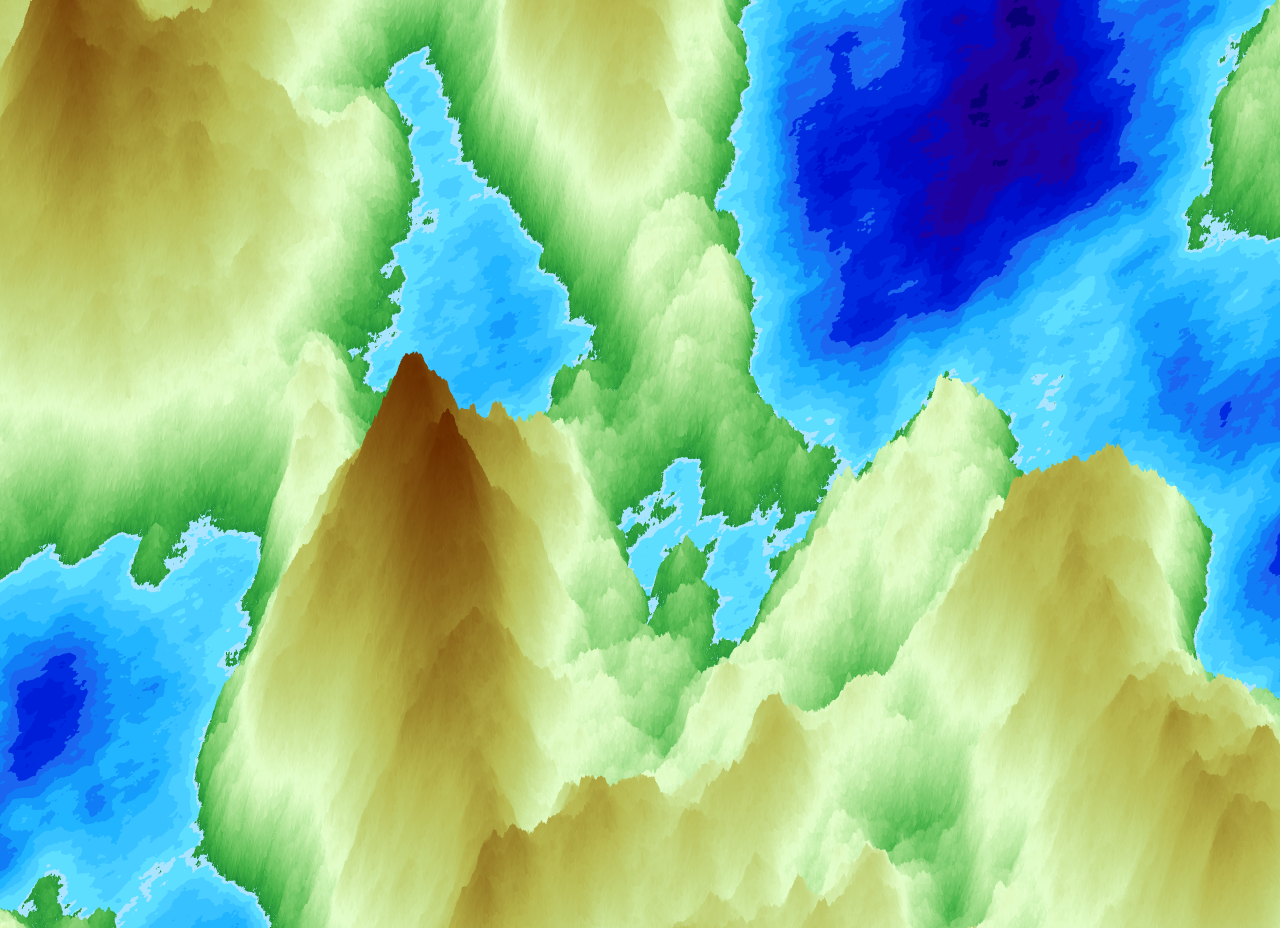
\includegraphics[width=\textwidth]{img/big.png}
    \caption{\label{fig:full} Detail of a terrain generated using different fractal algorithms. }
\end{figure}
\pagebreak
\FloatBarrier

\bibliographystyle{plain}
\renewcommand{\bibname}{References}
\bibliography{references}